\documentclass[11pt,a4paper]{article}

\usepackage[utf8]{inputenc}
\usepackage[T1]{fontenc}
\usepackage[spanish,es-tabla]{babel}
\usepackage{lmodern}
\usepackage{microtype}
\usepackage[a4paper,margin=2.35cm]{geometry}
\usepackage{amsmath,amssymb}
\usepackage{booktabs,tabularx,multirow,threeparttable}
\usepackage{graphicx}
\usepackage{caption}
\usepackage{subcaption}
\usepackage{placeins}
\usepackage{float}
\usepackage{xcolor}
\usepackage{enumitem}
\usepackage{tikz}
\usetikzlibrary{arrows.meta,positioning,fit,shapes.geometric}
\usepackage[numbers,sort&compress]{natbib}
\usepackage{hyperref}
\usepackage[nameinlink,noabbrev]{cleveref}

\definecolor{cbrblue}{HTML}{4C78A8}
\definecolor{mmrred}{HTML}{E45756}
\definecolor{ontogreen}{HTML}{54A24B}
\hypersetup{
  colorlinks=true,
  linkcolor=black,
  citecolor=cbrblue,
  urlcolor=cbrblue,
  pdftitle={De artículos científicos a recomendaciones CBR diversas: un pipeline auditado OntoCast--OPMAD para mantenimiento predictivo},
  pdfauthor={}
}
\captionsetup{font=small,labelfont=bf}
\setlist{nosep,leftmargin=*}
\newcommand{\OPMAD}{\textsc{opmad}}
\newcommand{\OntoCast}{\textsc{OntoCast}}
\newcommand{\myCBR}{myCBR}
\newcommand{\MMR}{\textsc{mmr}}
\newcommand{\RDF}{\textsc{rdf}}
\newcommand{\ILD}{\textsc{ild}}

\title{\textbf{De artículos científicos a recomendaciones CBR diversas: un pipeline auditado OntoCast--OPMAD para mantenimiento predictivo}}
\author{}
\date{}

\begin{document}
\maketitle

\begin{abstract}
La literatura científica de mantenimiento predictivo describe activos, señales, tareas y modelos que podrían alimentar sistemas de apoyo a decisiones (DSS, por \emph{decision-support systems}) basados en casos, pero convertir esos documentos en insumos estructurados, trazables y compatibles con infraestructuras heredadas sigue siendo difícil. Este trabajo presenta y audita un pipeline que parte de una búsqueda bibliográfica, procesa documentos con \OntoCast{} condicionado por \OPMAD{}, genera artefactos RDF/Turtle, los transforma a un esquema CBR de 19 campos, ejecuta consultas \myCBR{} y aplica reranking por relevancia marginal máxima (MMR) para reducir redundancia en las recomendaciones. De 3.990 registros Scopus publicados en 2025--2026, 2.768 cumplieron los criterios de inclusión; se recuperaron 1.822 PDF, correspondientes a 1.821 documentos únicos. Todos los documentos únicos generaron artefactos parseables tras limpieza RDF-star y consultas ejecutables contra una base histórica de 263 casos. Sin embargo, la auditoría reveló pérdidas semánticas importantes: varios campos quedaron como valores predeterminados o se descartaron durante la normalización, y solo 126/1.821 artefactos cumplieron las formas SHACL mínimas. En la tarea downstream, con pool 15, top-5 y $\lambda=0{,}70$, MMR incrementó la disimilitud intra-lista de 0,4216 a 0,5265 y redujo las listas con firmas de modelos repetidas de 610 a 5, con una reducción de similitud media top-5 de 0,5563 a 0,5536. Comparadores max-sum, MAP-DPP (\emph{maximum a posteriori determinantal point process}) y deduplicación exacta, junto con análisis de sensibilidad, muestran un compromiso configurable entre relevancia y diversidad, no una superioridad universal. La evidencia respalda interoperabilidad ejecutable y comportamiento algorítmico de ranking; no demuestra fidelidad factual de las extracciones ni utilidad decisional humana.
\end{abstract}

\noindent\textbf{Palabras clave:} extracción de información guiada por ontologías; mantenimiento predictivo; razonamiento basado en casos; grafos de conocimiento; modelos de lenguaje; recuperación con diversidad.

\begin{center}
\rule{0.92\linewidth}{0.4pt}
\end{center}

\begin{otherlanguage}{english}
\renewcommand{\abstractname}{Abstract}
\begin{abstract}
Predictive-maintenance papers describe assets, signals, tasks, and models that could feed case-based decision-support systems, but converting those documents into structured, traceable, and legacy-compatible inputs remains difficult. This study presents and audits a pipeline that starts from bibliographic search, processes documents with OPMAD-constrained \OntoCast{}, produces RDF/Turtle artifacts, maps them to a 19-field CBR schema, executes \myCBR{} queries, and applies maximal marginal relevance (MMR) reranking to reduce recommendation redundancy. From 3,990 Scopus records published in 2025--2026, 2,768 met the inclusion criteria; 1,822 PDFs were retrieved, corresponding to 1,821 unique documents. All unique documents yielded parseable artifacts after RDF-star cleanup and executable queries against a historical base of 263 cases. Field-level audits nevertheless revealed substantial semantic loss: several fields remained defaults or were discarded during normalization, and only 126/1,821 artifacts satisfied the minimal SHACL shapes. In the downstream task, with a pool of 15, top-5 output, and $\lambda=0.70$, MMR increased mean intra-list dissimilarity from 0.4216 to 0.5265 and reduced lists with repeated model signatures from 610 to 5, while mean top-5 similarity decreased from 0.5563 to 0.5536. Max-sum, MAP-DPP (maximum a posteriori determinantal point process), exact-deduplication comparators and sensitivity analyses show a configurable relevance--diversity trade-off rather than universal superiority. The evidence supports executable interoperability and algorithmic ranking behavior; it does not demonstrate factual extraction fidelity or human decision utility.

\textbf{Keywords:} ontology-guided information extraction; predictive maintenance; case-based reasoning; knowledge graphs; large language models; diversity-aware retrieval.
\end{abstract}
\end{otherlanguage}

\crefname{figure}{figura}{figuras}
\crefname{table}{tabla}{tablas}
\crefname{equation}{ecuación}{ecuaciones}
\crefname{section}{sección}{secciones}
\Crefname{figure}{Figura}{Figuras}
\Crefname{table}{Tabla}{Tablas}
\Crefname{equation}{Ecuación}{Ecuaciones}
\Crefname{section}{Sección}{Secciones}

\section{Introducción}
\label{sec:intro}

El mantenimiento predictivo organiza decisiones de intervención a partir de la condición y evolución esperada de un activo. Sus arquitecturas combinan adquisición, preprocesamiento, diagnóstico, pronóstico y comunicación; cada función admite modelos basados en conocimiento, datos o física y configuraciones multimodelo \citep{MonteroJimenez2020Survey}. Durante el diseño conceptual, esta amplitud dificulta seleccionar componentes y justificar alternativas.

En términos operativos, el problema estudiado es el siguiente: un artículo describe un activo, señales, una tarea y modelos; esos hechos deben convertirse en los atributos que entiende un sistema de razonamiento basado en casos (CBR) usado como sistema de apoyo a decisiones (DSS), el cual devuelve experiencias históricas y modelos candidatos. El CBR reutiliza experiencias mediante recuperación, reutilización, revisión y retención \citep{Aamodt1994CBR,LopezDeMantaras2005CBR}; una ontología puede aportar vocabulario, estructura y similitud semántica \citep{Gruber1993Ontology,AmailefLu2013OntologyCBR,Qin2018OntologyCBR}. La infraestructura previa basada en el modelo ontológico para arquitectura y diseño de mantenimiento predictivo (\OPMAD{}, por \emph{Ontology model for Predictive Maintenance Architecture and Design}) y en la plataforma \myCBR{} recomienda modelos de mantenimiento predictivo \citep{MonteroJimenez2021OPMADCBR,MunozHernandez2021OntologyCBR}, pero depende de incorporación manual y puede devolver soluciones homogéneas.

El estudio parte de tres observaciones. Primero, los modelos de lenguaje de gran tamaño (LLM, por \emph{large language models}) pueden extraer grafos desde texto \citep{Pan2024LLMKG,Lairgi2024IText2KG}, pero un archivo en Resource Description Framework (RDF) parseable no garantiza que los hechos sean correctos, completos o útiles para una herramienta de decisión. Segundo, si esos hechos se usarán en un sistema CBR existente, deben traducirse a un esquema fijo de atributos; en ese paso pueden aparecer pérdidas de información, valores predeterminados y normalizaciones discutibles. Tercero, una lista CBR ordenada solo por similitud puede repetir alternativas muy parecidas. La diversidad se trata aquí como una tarea downstream separada: el método de vecinos más cercanos condensados (CNN, por \emph{Condensed Nearest Neighbour}) modifica la memoria CBR \citep{MunozPena2025Diversity}; la relevancia marginal máxima (MMR, por \emph{maximal marginal relevance}) reordena reversiblemente un conjunto candidato \citep{CarbonellGoldstein1998MMR}; y familias como xQuAD (\emph{explicit Query Aspect Diversification}) o los procesos puntuales determinantes (DPP, por \emph{determinantal point processes}) representan otras formas de cubrir intenciones o subconjuntos \citep{Santos2010xQuAD,Gan2020DPP}.

El estudio no propone una ontología, un motor CBR ni un algoritmo de diversificación nuevos. Se evalúa una capa de interoperabilidad auditada para transformar artículos científicos recuperados desde un buscador bibliográfico en afirmaciones compatibles con \OPMAD{}, consultas ejecutables para un sistema \myCBR{} heredado y rankings con diversidad controlada. La validación factual externa queda fuera del alcance de este experimento; por tanto, las preguntas se formulan en términos de ejecutabilidad, pérdida de información y comportamiento downstream:

\begin{description}[style=nextline,leftmargin=1.5cm,labelwidth=1.2cm]
  \item[P1.] ¿Puede una cadena Scopus/PDF/\OntoCast{}--\OPMAD{} producir artefactos RDF y consultas \myCBR{} ejecutables para literatura reciente de mantenimiento predictivo?
  \item[P2.] ¿Qué información se conserva o se pierde al transformar esos artefactos en el esquema CBR de 19 campos y después en consultas normalizadas?
  \item[P3.] ¿Cómo cambia el ranking CBR al aplicar MMR y comparadores de diversidad sobre el mismo conjunto candidato, y cuán sensible es ese cambio a parámetros, atributos y valores predeterminados?
\end{description}

El aporte se organiza en cuatro elementos:

\begin{enumerate}[label=(\roman*)]
  \item un pipeline reproducible desde artefactos canónicos que conecta búsqueda bibliográfica, extracción \OntoCast{} condicionada por \OPMAD{}, artefactos RDF/Turtle, puente a 19 campos y consultas \myCBR{};
  \item una auditoría de cobertura, valores predeterminados, conformidad con Shapes Constraint Language (SHACL), limpieza RDF-star, selección de casos, normalización y atributos realmente activos en la consulta;
  \item una evaluación pareada de recuperación CBR y CBR+MMR sobre 1.821 consultas, con bootstrap por clúster, sensibilidad a parámetros y comparadores max-sum, MAP-DPP y deduplicación;
  \item un paquete de reproducción con manifiestos, hashes, resultados por consulta, scripts y amenazas explícitas sobre aquello que no se valida: fidelidad factual y utilidad humana.
\end{enumerate}

\section{Antecedentes y trabajos relacionados}
\label{sec:related}

\subsection{Ontologías y CBR en mantenimiento predictivo}

Una ontología formaliza conceptos y relaciones compartidos \citep{Gruber1993Ontology,NoyMcGuinness2001Ontology101}. En sistemas CBR, esa estructura ayuda a nombrar atributos, organizar casos y calcular similitudes más informadas que una comparación puramente léxica. Por ello, la integración entre ontologías y CBR se ha usado en dominios como emergencias, tolerancias, diseño y selección de procesos \citep{AmailefLu2013OntologyCBR,Qin2018OntologyCBR,RomeroBejarano2014CBRDesign,Mabkhot2019OntologyCBR}. En mantenimiento también existen grafos orientados a apoyar decisiones, por ejemplo para recomendar planes mediante redes neuronales de grafos \citep{Xia2023MaintenanceKG}.

En esta línea, \OPMAD{} ofrece un vocabulario especializado para artículos, activos, variables, modelos y funciones de mantenimiento predictivo. La infraestructura \OPMAD{}--\myCBR{} ya integra esa terminología con una base histórica de casos y funciones de similitud \citep{MonteroJimenez2021OPMADCBR,MunozHernandez2021OntologyCBR}. Por tanto, el presente trabajo no reclama novedad en la ontología, en la base de casos ni en el motor CBR. El problema abordado es otro: cómo poblar y evaluar esa representación a partir de literatura científica heterogénea con PDF accesible.

\subsection{Extracción estructurada con modelos de lenguaje}

Los modelos de lenguaje se han empleado para construir y completar grafos, alinear vocabularios y generar representaciones estructuradas a partir de texto \citep{Pan2024LLMKG}. iText2KG, por ejemplo, construye grafos de conocimiento de forma incremental \citep{Lairgi2024IText2KG}; otros trabajos guían al modelo con ontologías o automatizan mapeos hacia RDF \citep{Mustafa2025OntologyGuided,Marketakis2026RDFMappings}. \OntoCast{} se ubica en esta familia porque usa una ontología como restricción para producir hechos estructurados \citep{Belikov2025OntoCast}.

La dificultad no termina cuando se obtiene un grafo parseable. Un grafo puede estar bien formado y, aun así, omitir modelos, atribuir hechos a un trabajo citado, usar etiquetas demasiado genéricas o generar valores incompatibles con una aplicación downstream. Por eso, la evaluación debe separar al menos tres niveles: conformidad estructural, cobertura de campos y fidelidad semántica respecto del texto. En este manuscrito, la conformidad estructural se comprueba con formas SHACL mínimas \citep{SHACL2017}; la cobertura y la normalización se auditan campo por campo; y la fidelidad semántica se deja preparada como una etapa futura de anotación experta sobre evidencia textual congelada.

La población de ontologías y la extracción de información guiada por ontologías son áreas previas a los LLM y proporcionan criterios para separar entidades, relaciones, alineamiento y calidad de grafo \citep{WimalasuriyaDou2010OntologyIE,Petasis2011OntologyPopulation,Hogan2021KnowledgeGraphs,Zaveri2016LinkedDataQuality}. En artículos científicos, además, la extracción depende de segmentación, secciones, tablas y metadatos; corpus y modelos como S2ORC, SciIE o SciBERT ilustran esa familia de problemas \citep{Luan2018SciIE,Beltagy2019SciBERT,Lo2020S2ORC}. Alternativas como búsqueda semántica, RAG o KG-RAG podrían recuperar fragmentos o respuestas desde literatura \citep{Lewis2020RAG}; no se comparan aquí porque el objetivo es distinto: producir una consulta estructurada compatible con similitudes CBR heredadas y auditar las pérdidas del puente RDF--CBR.

\subsection{Recuperación y diversidad como tarea downstream}

La recuperación CBR se basa en similitud, pero una lista de casos muy similares puede ser poco útil si repite soluciones equivalentes. La literatura distingue por ello entre relevancia y diversidad \citep{SmythMcClave2001Diversity,McSherry2002Diversity}, y los sistemas de recomendación estudian medidas complementarias como cobertura, novedad o serendipia \citep{KaminskasBridge2016BeyondAccuracy}. En este manuscrito, la recuperación CBR no se usa como prueba de verdad factual; se usa como tarea downstream para observar qué ocurre cuando las afirmaciones extraídas se traducen a consultas.

Existen varias formas de introducir diversidad. La literatura de mantenimiento de bases de casos estudia competencia, edición y condensación de la memoria \citep{SmythMcKenna1999Competence}; en esa línea, el CNN modificado condensa o reorganiza la memoria de casos \citep{MunozPena2025Diversity}. En cambio, MMR penaliza la similitud con los elementos ya seleccionados y reordena un conjunto candidato sin modificar la base de casos \citep{CarbonellGoldstein1998MMR}. xQuAD representa explícitamente aspectos o intenciones de búsqueda \citep{Santos2010xQuAD}, mientras que los DPP favorecen subconjuntos diversos mediante un determinante \citep{Gan2020DPP}. Por esa diferencia conceptual, el reranking se interpreta aquí como análisis secundario de uso downstream, no como contribución principal de extracción.

\begin{table}[H]
\centering
\caption{Posicionamiento del estudio respecto de familias próximas.}
\label{tab:positioning}
\footnotesize
\begin{tabularx}{\linewidth}{lXXX}
\toprule
Familia & Pregunta típica & Evidencia habitual & Papel en este estudio \\
\midrule
Modelos de lenguaje y grafos & ¿se puede estructurar texto como grafo? & triples, clases o relaciones & se evalúa además cobertura, trazabilidad y uso downstream \\
Ontología--CBR & ¿mejora una ontología la recuperación de casos? & similitud, competencia o utilidad & se reutiliza \OPMAD{}--\myCBR{} como infraestructura existente \\
Grafos de mantenimiento & ¿apoyan decisiones sobre activos? & desempeño en una tarea industrial & se usan como referencia conceptual, no como predictor \\
Diversificación & ¿la lista recuperada cubre alternativas? & relevancia y diversidad & se analiza como tarea secundaria posterior a la extracción \\
\bottomrule
\end{tabularx}
\end{table}

\begin{table}[H]
\centering
\caption{Delimitación de componentes reutilizados y aportes de este trabajo.}
\label{tab:component-boundary}
\footnotesize
\begin{tabularx}{\linewidth}{lXXX}
\toprule
Componente & Estado previo & Nuevo en este trabajo & Evidencia reportada \\
\midrule
OPMAD & ontología de dominio existente & uso como restricción fija de extracción & semilla, SHACL y cobertura por campo \\
\myCBR{} y base de casos & DSS heredado con 263 casos & ejecución por lotes desde consultas extraídas & 1.821 consultas y ablaciones \\
\OntoCast{} & extractor externo & aplicación condicionada por \OPMAD{} en corpus PdM & artefactos RDF y auditoría de lotes/modelos \\
Puente RDF--CBR & no disponible para el corpus & conversión determinista a 19 campos y normalización & defaults, campos activos y pérdidas \\
MMR/diversidad & algoritmo estándar & capa reversible sobre pool CBR sin modificar memoria & comparadores, sensibilidad y bootstrap por clúster \\
\bottomrule
\end{tabularx}
\end{table}

\section{Materiales y métodos}
\label{sec:methods}

\subsection{Diseño del estudio}

Se realizó un experimento computacional de evaluación de pipeline. La unidad de análisis fue un documento científico único con un artefacto de extracción asociado. Para cada documento se siguió la misma cadena: extracción de afirmaciones condicionada por \OPMAD{}, limpieza y conversión al esquema de 19 campos, normalización de los campos que puede usar \myCBR{} y generación de una consulta contra la base histórica de 263 casos. De esta forma, cada documento produjo una representación estructurada y una consulta comparable con las demás.

La comparación de recuperación fue pareada porque la misma consulta se evaluó en dos condiciones: (a) el top-5 devuelto directamente por \myCBR{} ordenado por similitud, usado como línea base (\emph{baseline}); y (b) un top-5 reordenado con MMR a partir de los 15 candidatos más similares. Este diseño mantiene constante la extracción, el puente RDF--CBR, la base de casos y la consulta; solo cambia la regla que selecciona la lista final desde el conjunto candidato. Por ello, las diferencias observadas en similitud y diversidad se interpretan como efecto del reranking, no como diferencias entre documentos o entre extracciones.

Además de esa comparación downstream, se realizaron auditorías de interoperabilidad y trazabilidad: cobertura de los 19 campos, conformidad SHACL, uso de valores predeterminados, normalización hacia el vocabulario histórico, modelo de lenguaje que generó cada artefacto, confianza del enlace PDF--facts, atributos activos en la consulta CBR y sensibilidad a parámetros de reranking. El estudio no entrenó un predictor, no evaluó diagnóstico o pronóstico industrial real y no midió utilidad humana. La fidelidad factual de las extracciones queda fuera del alcance de este experimento computacional.

\subsection{Corpus y cribado}

El corpus se construyó a partir de registros Scopus en inglés publicados en 2025--2026. La estrategia de búsqueda combinó términos de mantenimiento predictivo, mantenimiento basado en condición, pronóstico y salud de sistemas, estimación de vida útil remanente, monitorización de condición y pronóstico de fallas. Para reducir ruido, se excluyeron revisiones y usos ambiguos de acrónimos frecuentes. El cribado aplicó dos criterios de inclusión simultáneos: el artículo debía referirse a un activo físico diseñado y debía tener un propósito explícito de mantenimiento, inspección, diagnóstico, pronóstico o decisión basada en condición.

El flujo de selección separó tres etapas: recuperación bibliográfica, cribado temático y disponibilidad de texto completo. De 3.990 registros recuperados, 2.768 cumplieron los criterios de inclusión y 1.222 fueron excluidos. Para los registros incluidos se intentó recuperar el PDF por vías legales; se obtuvieron 1.822 archivos, de los cuales dos correspondían al mismo contenido, por lo que el análisis usa 1.821 documentos únicos. Los 946 registros incluidos sin PDF accesible no se trataron como fallos de extracción, sino como una fuente de sesgo de cobertura: la disponibilidad de texto completo varió por año y por modalidad de acceso. La \cref{fig:flow-corpus} resume el flujo; la consulta Scopus, las decisiones de cribado por registro y la auditoría de disponibilidad se documentan en el suplemento.

\begin{figure}[t]
\centering
\begin{tikzpicture}[
  node distance=5mm and 7mm,
  box/.style={draw,rounded corners,align=center,minimum width=2.45cm,minimum height=1.0cm,fill=gray!6,font=\small},
  keep/.style={box,fill=ontogreen!12},
  arrow/.style={-{Latex[length=2mm]},thick}
]
\node[box] (scopus) {Scopus\\3.990 registros};
\node[keep,right=of scopus] (screen) {Cribado\\2.768 incluidos};
\node[box,below=of screen] (excluded) {1.222 excluidos};
\node[keep,right=of screen] (pdf) {1.822 PDF\\recuperados};
\node[keep,right=of pdf] (unique) {1.821 documentos\\únicos};
\node[keep,right=of unique] (facts) {1.821 artefactos\\RDF y consultas};
\draw[arrow] (scopus) -- (screen);
\draw[arrow] (screen) -- (pdf);
\draw[arrow] (pdf) -- (unique);
\draw[arrow] (unique) -- (facts);
\draw[arrow] (screen) -- (excluded);
\node[below=2mm of pdf,font=\scriptsize,align=center,text width=2.6cm] {946 incluidos sin PDF accesible};
\end{tikzpicture}
\caption{Flujo del corpus experimental. La diferencia entre 1.822 archivos y 1.821 documentos se debe a un duplicado exacto, no a una extracción ausente.}
\label{fig:flow-corpus}
\end{figure}

\subsection{Extracción condicionada por OPMAD}

Los documentos se procesaron por lotes con modelos GPT mediante \OntoCast{} en modo de ontología fija. La extracción usó una semilla autocontenida de \OPMAD{} (56 clases, 15 propiedades de objeto y dos propiedades de datos) para restringir el vocabulario a artículos, activos, variables, modelos y funciones de mantenimiento. En esta configuración, \OntoCast{} no debía crear clases nuevas ni modificar la ontología; debía generar, para cada documento, un archivo Turtle con afirmaciones compatibles con \OPMAD{}.

El corpus final combina tres lotes históricos: gpt-5-mini (599 artefactos), gpt-5.4-mini (500) y gpt-5.6-luna (722). Esta mezcla se trata como una amenaza de validez y no como factor experimental aleatorizado. La entrada al extractor no debe interpretarse como lectura exhaustiva del PDF completo: 1.802 documentos se procesaron con tres fragmentos iniciales y 19 con un fragmento. Por ello, campos ubicados típicamente en métodos, resultados o tablas pueden quedar ausentes aunque existan en el artículo.

Esos archivos Turtle fueron la entrada del puente RDF--CBR descrito en la siguiente subsección. La limpieza retiró bloques RDF-star incompatibles con el parser RDF 1.1 para poder calcular las consultas; las asociaciones extraídas se preservaron en un sidecar para auditoría, pero no se usaron como criterio de similitud ni como prueba de fidelidad semántica.

\subsection{Puente RDF--CBR y normalización}

El archivo \texttt{facts\_to\_csv.py} actúa como puente entre las afirmaciones RDF y el esquema CBR. Para cada archivo Turtle, el puente lee el grafo, identifica entidades por tipo y recupera sus nombres mediante etiquetas como \texttt{schema:name} y \texttt{rdfs:label}. Después transforma la información disponible en una fila validada por un modelo Pydantic de 19 campos. Esos campos agrupan metadatos bibliográficos, tarea de mantenimiento, activo, señales o variables de entrada, preprocesamiento, configuración y nombres de modelos, sincronización, modos de falla, desempeño y notas complementarias.

Cuando el grafo no contiene evidencia para un campo, el puente usa marcas explícitas de ausencia, por ejemplo \texttt{Not reported} o \texttt{Unknown synchronization}; algunos campos numéricos heredados se completan con cero. Estos valores permiten construir archivos CSV válidos y consultas ejecutables, pero no deben interpretarse como hechos extraídos del texto. Por esa razón, la auditoría distingue entre valores informativos, valores predeterminados y etiquetas genéricas generadas automáticamente.

Cada documento se procesó de forma independiente. Si un archivo Turtle contenía más de un posible caso, se seleccionó un caso de manera determinista, por orden de identificador internacionalizado de recurso (IRI, por \emph{Internationalized Resource Identifier}), para evitar duplicar el documento, aunque esa regla no garantiza siempre que el caso elegido corresponda al estudio fuente. Antes de consultar \myCBR{}, los valores se alinearon con el vocabulario histórico de la base de casos; los campos no reconocidos o los valores predeterminados sin evidencia se descartaron o recibieron peso cero. La conformidad estructural se revisó con formas SHACL mínimas sobre título, modelos, activos y variables. Esta validación comprueba que el artefacto tiene la estructura esperada, pero no demuestra exactitud factual respecto del texto.

\subsection{Recuperación CBR}

Las consultas normalizadas se ejecutaron contra la base histórica \myCBR{} utilizada en la infraestructura \OPMAD{}--CBR. Esta base contiene 263 casos documentados de aplicaciones de modelos en mantenimiento predictivo. Para evitar inconsistencias entre la recuperación y el análisis posterior, la misma versión de la base se usó tanto para consultar casos como para leer las firmas de solución empleadas en las métricas de diversidad. Los documentos extraídos pertenecen a 2025--2026, mientras que los casos históricos son anteriores; por ello, la evaluación mantiene una separación temporal entre literatura objetivo y memoria CBR.

Cada consulta contiene únicamente los atributos que sobrevivieron al puente y a la normalización. \myCBR{} calcula la similitud global a partir de similitudes locales para tarea, tipo y nombre del activo, sincronización, modalidad, variables de entrada y año. La tarea utiliza relaciones ontológicas, el nombre del activo se compara mediante distancia de Levenshtein y las variables de entrada se tratan como conjuntos; otros atributos emplean tablas simbólicas heredadas de la infraestructura previa \citep{Sanchez2012SemanticSimilarity,MonteroJimenez2021OPMADCBR}. Los atributos vacíos no aportan peso a la consulta, y los valores usados solo como marcas de ausencia no se trataron como evidencia.

La salida directa de \myCBR{} se usó como línea base: los cinco casos más similares forman el top-5 sin diversificación. Para la condición con diversidad, primero se recuperó un conjunto candidato de 15 casos y después se aplicó el reranking descrito en la siguiente subsección. El año de consulta se fijó en 2026 para mantener constante la función de recencia. Como controles de sensibilidad se evaluaron consultas con diferentes subconjuntos de atributos y años alternativos, con el fin de identificar qué parte del ranking dependía de tarea, activo, variables o recencia.

\subsection{Reranking MMR}
\label{sec:mmr}

El reranking se añadió como postproceso de la recuperación CBR. Su objetivo no es cambiar la similitud calculada por \myCBR{} ni modificar la base de casos, sino seleccionar una lista final menos redundante a partir de un conjunto candidato ya recuperado. En términos prácticos, cada consulta produce primero un pool de casos similares; después MMR escoge una lista corta que balancea dos criterios: conservar casos relevantes para la consulta y evitar soluciones demasiado parecidas entre sí.

Para medir si dos recomendaciones son parecidas se definió una similitud de solución, $s_{\mathrm{sol}}$. Esta función no compara los problemas descritos por los artículos, sino las soluciones recomendadas por la base CBR. Combina cuatro componentes: enfoque del modelo, tipo de modelo, nombres de modelos y preprocesamiento:
\begin{equation}
 s_{\mathrm{sol}}(x,y)=0{,}20s_{\mathrm{enfoque}}+0{,}25s_{\mathrm{tipo}}+0{,}40s_{\mathrm{modelos}}+0{,}15s_{\mathrm{prep}}.
 \label{eq:solution-sim}
\end{equation}
El mayor peso se asignó a los nombres de modelos porque el objetivo de la diversificación era reducir listas con alternativas modelísticas repetidas. Para enfoque y tipo se combinaron coincidencias léxicas; para modelos se añadió una taxonomía de términos de la base histórica; y para preprocesamiento se usó coincidencia exacta. Cuando una recomendación enumera varios algoritmos en el campo \texttt{Models}, la firma de modelos se interpreta como una cadena multivalor normalizada, no como un único algoritmo. Estas firmas provienen de los casos históricos recomendados por \myCBR{}, no necesariamente de los modelos extraídos del artículo usado como consulta.

MMR selecciona los elementos de forma voraz. El primer resultado de \myCBR{} se conserva para no alterar la recomendación más similar. Luego, cada nuevo elemento se elige maximizando:
\begin{equation}
 x^{*}=\arg\max_{x\in R\setminus S}\left[\lambda\,\mathrm{rel}(x)-(1-\lambda)\max_{y\in S}s_{\mathrm{sol}}(x,y)\right],
 \label{eq:mmr}
\end{equation}
donde $R$ es el pool candidato, $S$ la lista ya seleccionada y $\mathrm{rel}(x)$ la similitud global calculada por \myCBR{}. El parámetro $\lambda$ controla el compromiso: valores altos priorizan relevancia CBR y valores bajos penalizan con más fuerza la redundancia entre soluciones. La configuración principal usó $\lambda=0{,}70$, pool 15 y salida top-5.

Para comprobar que las conclusiones no dependieran de una sola parametrización, se evaluaron valores alternativos de $\lambda$, tamaños de pool, tamaños de lista y pesos de $s_{\mathrm{sol}}$. También se comparó MMR con reglas que responden a criterios diferentes: deduplicación exacta de firmas de modelos, selección max-sum y MAP-DPP (\emph{maximum a posteriori} sobre un proceso puntual determinantal). Estos comparadores no se presentan como métodos nuevos; sirven para mostrar si la reducción de redundancia observada es propia de MMR o del objetivo de diversidad elegido.

\begin{figure}[H]
\centering
\begin{tikzpicture}[
  node distance=6mm and 7mm,
  proc/.style={draw,rounded corners,align=center,minimum width=2.25cm,minimum height=1.05cm,fill=gray!6,font=\small},
  data/.style={proc,fill=cbrblue!10},
  sem/.style={proc,fill=ontogreen!12},
  rank/.style={proc,fill=mmrred!10},
  arrow/.style={-{Latex[length=2mm]},thick}
]
\node[data] (pdf) {PDF};
\node[sem,right=of pdf] (cast) {\OntoCast{}\\\OPMAD{} fija};
\node[data,right=of cast] (rdf) {Hechos RDF-star\\por documento};
\node[sem,right=of rdf] (bridge) {Limpieza + puente\\19 campos};
\node[data,below=of bridge] (query) {Consulta\\normalizada};
\node[proc,left=of query] (cbr) {\myCBR{}\\pool top-15};
\node[rank,left=of cbr] (mmr) {MMR\\top-5};
\node[sem,below=of cbr] (base) {Base OPMAD\\263 casos};
\node[sem,below=of mmr] (tax) {Taxonomía\\131 términos};
\draw[arrow] (pdf) -- (cast);
\draw[arrow] (cast) -- (rdf);
\draw[arrow] (rdf) -- (bridge);
\draw[arrow] (bridge) -- (query);
\draw[arrow] (query) -- (cbr);
\draw[arrow] (cbr) -- (mmr);
\draw[arrow] (base) -- (cbr);
\draw[arrow] (tax) -- (mmr);
\end{tikzpicture}
\caption{Arquitectura evaluada. El reranking no modifica la base de casos ni los puntajes CBR; selecciona cinco recomendaciones desde el pool de 15.}
\label{fig:architecture}
\end{figure}

\subsection{Alcance de la validación semántica}
\label{sec:semantic-scope}

Este estudio no ejecuta una validación factual externa. Por tanto, las métricas reportadas no deben interpretarse como precisión, exhaustividad o utilidad experta de las extracciones. La unidad experimental es un artefacto computacional que puede transformarse en consulta y ranking; no es un caso validado para retención automática en la memoria CBR.

Para mantener la frontera metodológica clara, los análisis se limitan a cuatro niveles: parseabilidad de los artefactos después de la limpieza RDF-star, cobertura no predeterminada del esquema de 19 campos, supervivencia de atributos durante la normalización hacia \myCBR{} y comportamiento de rankings antes y después del reranking. Una futura evaluación semántica debería comparar valores extraídos contra evidencia textual congelada y anotar campos como tarea, activo, variables, modelos, sincronización, modos de falla y desempeño; esa fase no forma parte de los resultados aquí presentados.

\subsection{Métricas y análisis estadístico}

Las métricas se organizaron en tres grupos. El primero evalúa interoperabilidad: número de documentos con artefactos parseables, número de consultas ejecutables, cobertura no predeterminada de los campos del esquema y conformidad estructural mediante SHACL. Estas métricas indican si la cadena produce objetos computables, pero no demuestran que los valores sean correctos respecto del texto.

El segundo grupo describe la recuperación CBR antes y después del reranking. Para cada consulta se registró la similitud del primer resultado, la similitud media del top-5, el número de firmas de modelos distintas, la presencia de firmas repetidas, los cambios de orden y los cambios de conjunto. Estas medidas permiten observar si el postproceso modifica la lista final y cuánto cuesta esa modificación en términos de similitud CBR.

El tercer grupo mide diversidad algorítmica mediante disimilitud intra-lista (ILD, por \emph{intra-list dissimilarity}). Para una lista $L$ de $k=5$ recomendaciones, se calculó:
\begin{equation}
 \ILD(L)=\frac{2}{k(k-1)}\sum_{i<j}\left[1-s_{\mathrm{sol}}(x_i,x_j)\right],\qquad k=5.
 \label{eq:ild}
\end{equation}
Esta métrica usa la misma similitud de solución definida para MMR en la \cref{eq:solution-sim}. Por tanto, debe interpretarse como una medida alineada con el objetivo del reranking, no como validación independiente de utilidad, novedad percibida o calidad técnica de los modelos recomendados.

El análisis principal fue pareado: para cada documento se comparó la lista top-5 de \myCBR{} con la lista top-5 obtenida después de MMR. Se reportaron diferencias medias e intervalos de confianza del 95\% mediante 20.000 remuestras bootstrap. Como muchas consultas pueden producir rankings idénticos o muy parecidos, se repitió el bootstrap agrupando por firmas normalizadas y por patrones de ranking; así se evitó tratar rankings duplicados como evidencia completamente independiente.

Los análisis de sensibilidad evaluaron cambios en $\lambda$, tamaño del pool, tamaño de la lista, pesos de la similitud de solución, atributos activos de la consulta y año usado por la función de recencia. Las pruebas estadísticas no se interpretan como inferencia sobre una población clínica o industrial, sino como estabilidad del comportamiento algorítmico bajo el corpus estudiado. La fidelidad semántica de extracción queda fuera de este experimento y no se reemplaza por un juez LLM.

\section{Resultados}
\label{sec:results}

\subsection{Ejecutabilidad y cobertura del esquema}

El primer resultado evaluado fue si la extracción condicionada por \OPMAD{} podía convertirse en una representación computable para el flujo downstream. Los 1.821 documentos únicos produjeron artefactos procesables y consultas que \myCBR{} pudo ejecutar con al menos cinco casos recuperados. Este resultado confirma que la cadena técnica es operativa, pero no debe confundirse con calidad factual: una consulta ejecutable puede estar basada en pocos campos, en valores genéricos o en información parcial.

La auditoría identificó límites importantes. Todos los artefactos fueron parseables solo después de retirar 311.559 bloques de reificación RDF-star; esas asociaciones quedaron en un sidecar, no en el grafo limpio usado por el puente. Además, 409 artefactos contenían más de un posible caso y se ignoraron 567 casos adicionales para mantener una consulta por documento. La validación SHACL mínima fue conforme en 126/1.821 artefactos; las violaciones se concentraron en modelos, activos y variables, por lo que SHACL se interpreta como diagnóstico estructural y no como prueba de fidelidad.

La auditoría por campo muestra la diferencia entre compatibilidad sintáctica y contenido útil. Los elementos más cercanos a la recuperación CBR aparecieron con mayor frecuencia: tarea, activo, variables de entrada y modelos. En cambio, tipo de activo, sincronización, modos de falla, indicadores de desempeño y desempeño quedaron ausentes o representados por valores predeterminados en todos los documentos. La \cref{tab:coverage} resume campos críticos y la \cref{fig:field-coverage} muestra la cobertura no predeterminada completa. Así, el esquema de 19 campos funcionó como destino de interoperabilidad, pero no todos sus campos recibieron evidencia útil con la misma frecuencia.

\begin{table}[H]
\centering
\caption{Cobertura informativa y atributos activos después de la normalización ($n = 1\,821$).}
\label{tab:coverage}
\footnotesize
\begin{tabularx}{\linewidth}{lrrrX}
\toprule
Campo & Info. & \% & Activo en query & Observación \\
\midrule
Task & 1.727 & 94,8 & 1.821 & 94 casos recibieron tarea predeterminada \\
Case study & 1.544 & 84,8 & 1.549 & principal atributo textual \\
Input type & 1.301 & 71,4 & 1.381 & listas normalizadas de variables/señales \\
Models & 1.395 & 76,6 & --- & usado para auditar solución, no como atributo de consulta \\
Model type & 1.296 & 71,2 & --- & usado en firmas de solución \\
Input for model & 23 & 1,3 & 0 & descartado por incompatibilidad léxica \\
Case study type & 0 & 0,0 & 0 & valor genérico \texttt{Maintainable item} \\
Online/Off-line & 0 & 0,0 & 0 & \texttt{Unknown synchronization} tratado como ausente \\
Failure modes / performance & 0 & 0,0 & --- & no informativos en el puente actual \\
\bottomrule
\end{tabularx}
\end{table}

La tarea quedó activa en todas las consultas, pero en 94 documentos no hubo evidencia suficiente y se asignó el valor predeterminado \emph{One step future state forecast}; por ello, los resultados por tarea, especialmente ese estrato, se interpretan con cautela. Además, que un campo esté activo en la consulta no implica siempre evidencia fuerte: algunos valores débiles o derivados, incluidas etiquetas técnicas del tipo 	exttt{Facts*}, sobrevivieron a la normalización.

La normalización hacia el vocabulario histórico redujo aún más la información que efectivamente participó en la consulta. Algunos valores extraídos no coincidían con las categorías o formatos esperados por la base \myCBR{} y fueron descartados o tratados como ausentes. Como consecuencia, muchas consultas quedaron descritas por combinaciones simples de tarea, activo y variables, mientras que otras se aproximaron a una consulta mínima basada en tarea y año. Este resultado identifica un cuello de botella central del método: la extracción puede producir valores textuales plausibles, pero el sistema downstream solo aprovecha aquellos que sobreviven al mapeo y a la normalización.

\begin{figure}[H]
\centering
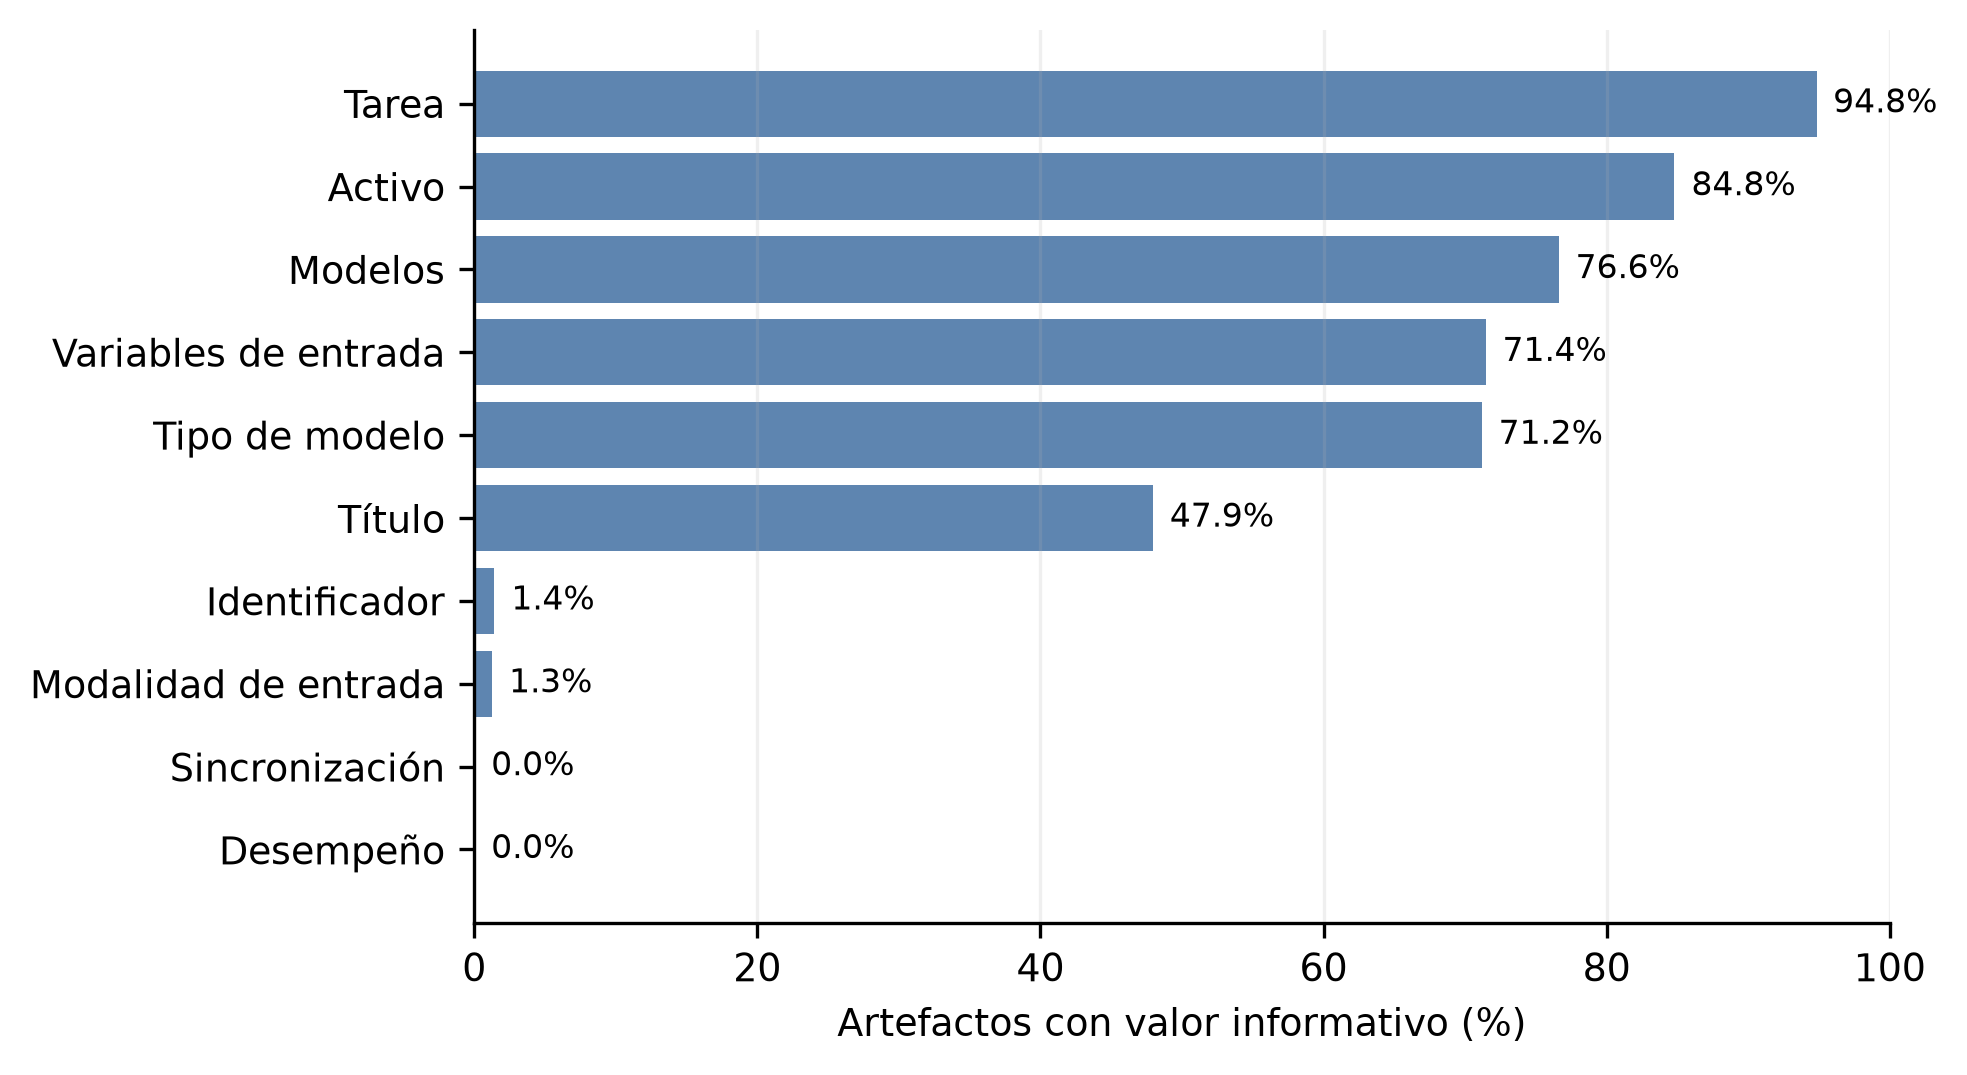
\includegraphics[width=0.74\linewidth]{figures/cobertura_campos.pdf}
\caption{Cobertura no predeterminada de campos seleccionados del puente. ``Informativo'' significa no genérico/no generado; no implica que el valor sea correcto respecto del texto fuente.}
\label{fig:field-coverage}
\end{figure}

\subsection{Efecto global del reranking}

La \cref{tab:main-results} y la \cref{fig:global-results} muestran el análisis principal. MMR elevó la \ILD{} 0,1049 (24,89\%); 1.707 consultas mejoraron, 112 disminuyeron y dos empataron. Las listas repetidas bajaron de 610 a 5 y las firmas distintas de modelos recomendados por la base histórica pasaron de 4,6332 a 4,9973. La similitud top-5 descendió 0,0027 (0,48\%); al excluir el top-1 fijado, el cambio en posiciones 2--5 fue $-0,0033$. El conjunto cambió en 1.819 consultas. El IC por consulta de \ILD{} fue [0,1013; 0,1087], pero al remuestrear los 848 rankings baseline se amplió a [0,0873; 0,1226]; para similitud fue [$-0,0033$; $-0,0021$].

\begin{table}[H]
\centering
\begin{threeparttable}
\caption{Resultados pareados principales ($n = 1\,821$, $\lambda=0{,}70$).}
\label{tab:main-results}
\small
\begin{tabular}{lrrrr}
\toprule
Métrica algorítmica & CBR & CBR+MMR & Cambio medio & IC del 95\% por clúster \\
\midrule
Similitud top-1 & 0,5630 & 0,5630 & 0,0000 & [0,0000; 0,0000] \\
Similitud media top-5 & 0,5563 & 0,5536 & $-0,0027$ & [$-0,0033$; $-0,0021$] \\
Firmas de modelos únicas & 4,6332 & 4,9973 & 0,3641 & [0,2720; 0,4678] \\
Listas con firma repetida & 610 & 5 & $-605$ & --- \\
Disimilitud intra-lista & 0,4216 & 0,5265 & 0,1049 & [0,0873; 0,1226] \\
\bottomrule
\end{tabular}
\begin{tablenotes}[flushleft]\footnotesize
\item Los intervalos tabulados remuestrean patrones de ranking baseline, una opción conservadora frente a rankings repetidos. El top-1 se fija por diseño.
\end{tablenotes}
\end{threeparttable}
\end{table}

\begin{figure}[H]
\centering
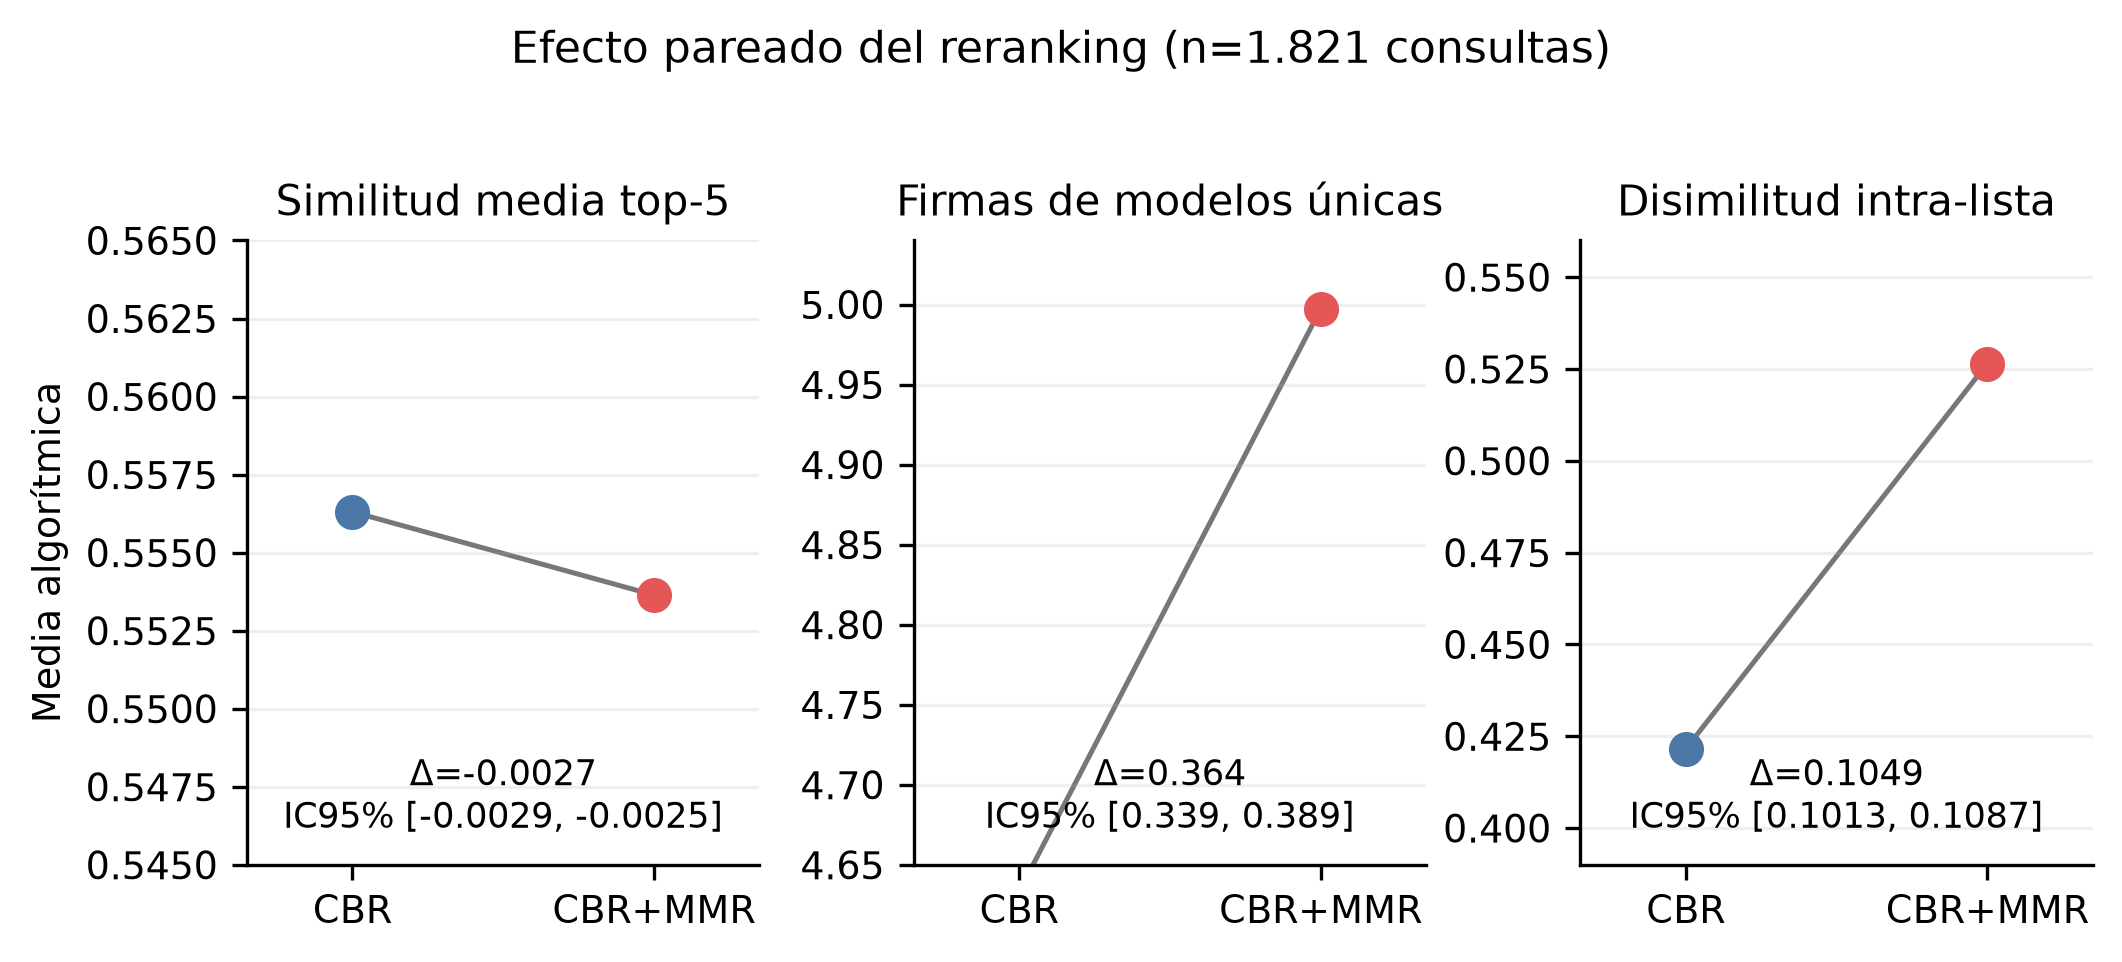
\includegraphics[width=\linewidth]{figures/metricas_globales.pdf}
\caption{Medias globales y cambio pareado. Cada panel usa escala propia.}
\label{fig:global-results}
\end{figure}

\begin{figure}[H]
\centering
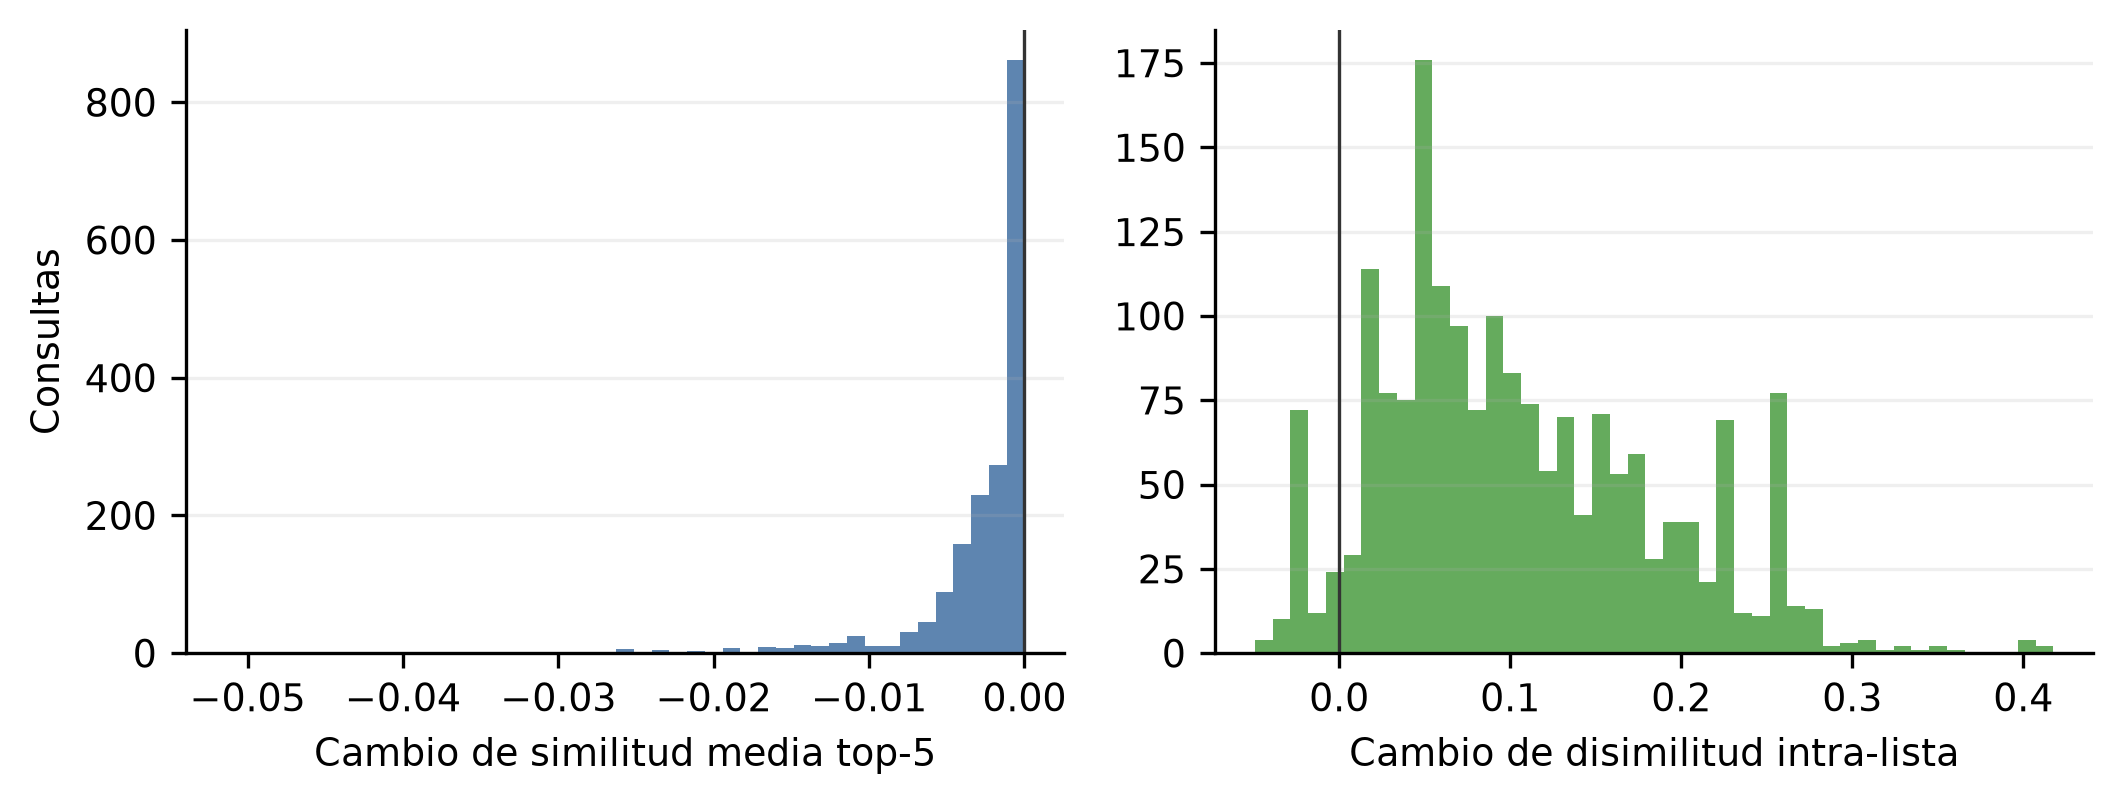
\includegraphics[width=0.92\linewidth]{figures/distribucion_cambios.pdf}
\caption{Distribución por consulta. El 5\% inferior del cambio de \ILD{} fue $-0,0146$ y el 95\% superior 0,2541; una media positiva no implica mejora en cada consulta.}
\label{fig:delta-distributions}
\end{figure}

\subsection{Comparadores, valores predeterminados y atributos CBR}

La \cref{tab:baselines} evita interpretar MMR como ganador universal. Deduplicar elimina todas las firmas repetidas con pérdida mínima, pero separa poco las soluciones. Max-sum logra la mayor \ILD{} según $s_{\mathrm{sol}}$, aunque conserva 35 listas repetidas. MAP-DPP logra cinco firmas exactas y la mayor cobertura de tipos (3,091), pero menor \ILD{} que MMR. Así, el método preferible depende del constructo: firmas, tipos o distancia compuesta.

\begin{table}[H]
\centering
\caption{Comparadores sobre el mismo pool 15 y top-1 fijo.}
\label{tab:baselines}
\footnotesize
\begin{tabular}{lrrrrr}
\toprule
Método & Sim. & \ILD{} & Firmas & Tipos & Repetidas \\
\midrule
CBR top-5 & 0,5563 & 0,4216 & 4,633 & 2,416 & 610 \\
Deduplicación & 0,5557 & 0,4373 & 5,000 & 2,544 & 0 \\
MMR ($\lambda=0{,}70$) & 0,5536 & 0,5265 & 4,997 & 2,881 & 5 \\
Max-sum ($\lambda=0{,}70$) & 0,5542 & 0,5408 & 4,980 & 2,789 & 35 \\
MAP-DPP léxico & 0,5540 & 0,4981 & 5,000 & 3,091 & 0 \\
\bottomrule
\end{tabular}
\end{table}

Ponderar \texttt{Unknown synchronization} cambió el top-1 en 483 consultas y dejó iguales 60,24\% de rankings MMR; se mantuvo como control. Las ablaciones mostraron que tarea+año colapsó el baseline a ocho rankings y cambió 1.361 top-1; tarea+variables produjo 16 rankings y cambió 1.355, mientras tarea+activo cambió solo seis top-1. Sin tarea, 270 consultas no devolvieron cinco casos. Fijar el año en 2021 cambió 593 top-1 y elevó artificialmente la similitud a 0,7695; 2025--2027 dieron el mismo ranking en esta función heredada.

\subsection{Sensibilidad a \texorpdfstring{$\lambda$}{lambda} y tareas}

La \cref{tab:sensitivity} confirma el intercambio esperado. Con 0,5 y 0,6 hubo cinco firmas en todas las listas; al elevar $\lambda$ reaparecieron repeticiones. El extremo $\lambda=0$ maximiza la penalización de redundancia dentro del pool y $\lambda=1$ reproduce el baseline. La configuración 0,70 fue preespecificada, no estimada como óptimo; 0,60 ofrece más firmas con similitud próxima.

\begin{table}[H]
\centering
\caption{Sensibilidad exacta del reranking (pool 15, top-5, top-1 fijo).}
\label{tab:sensitivity}
\small
\begin{tabular}{rrrrrr}
\toprule
$\lambda$ & Similitud media & Firmas únicas & Listas repetidas & \ILD{} & Conjunto cambiado \\
\midrule
0,0 & 0,5286 & 5,000 & 0  & 0,5418 & 1.821 \\
0,5 & 0,5522 & 5,000 & 0  & 0,5295 & 1.821 \\
0,6 & 0,5533 & 5,000 & 0  & 0,5274 & 1.821 \\
0,7 & 0,5536 & 4,997 & 5  & 0,5265 & 1.819 \\
0,8 & 0,5543 & 4,992 & 14 & 0,5248 & 1.818 \\
0,9 & 0,5549 & 4,986 & 25 & 0,5201 & 1.798 \\
1,0 & 0,5563 & 4,633 & 610 & 0,4216 & 0 \\
\bottomrule
\end{tabular}
\end{table}

Aumentar el pool de 10 a 30 redujo la similitud de 0,5546 a 0,5517 y elevó \ILD{} de 0,5037 a 0,5774 (\cref{fig:pool}); las listas repetidas bajaron de 11 a una. Con pesos uniformes, dominantes en modelos o sin preprocesamiento, la \ILD{} principal fue 0,5241, 0,5214 y 0,5165 frente a 0,5265; la similitud quedó entre 0,5536 y 0,5538. Quitar la restricción top-1 no cambió la salida: la primera selección de MMR sigue siendo el elemento de mayor relevancia cuando $S$ está vacío. El patrón se repitió para $k=3,5,10$; el suplemento contiene la cuadrícula completa.

\begin{figure}[H]
\centering
\begin{subfigure}[t]{0.49\linewidth}
  \centering
  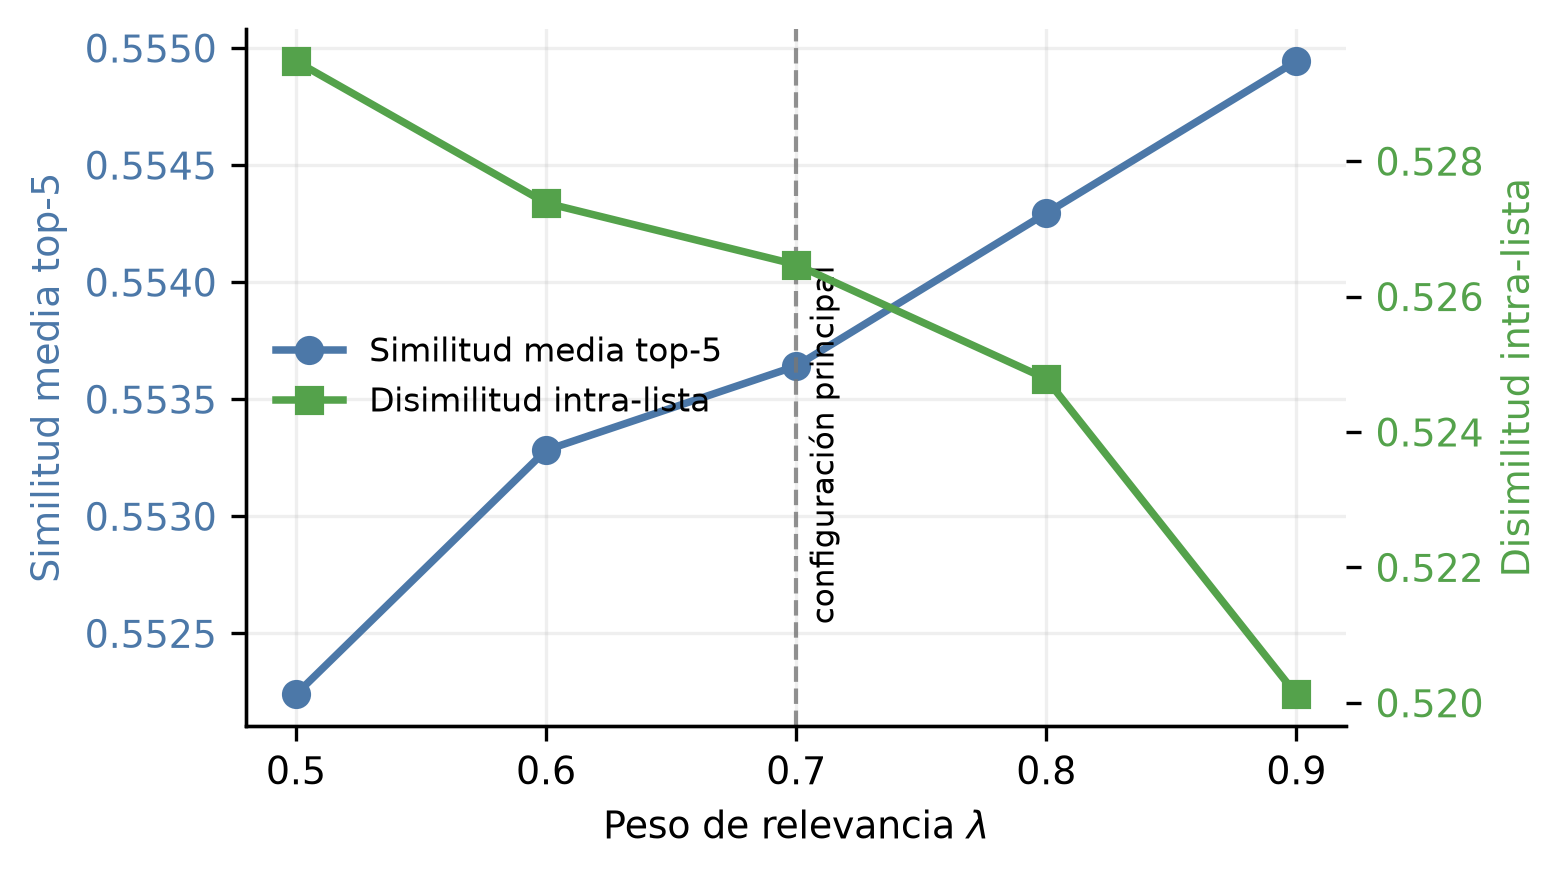
\includegraphics[width=\linewidth]{figures/sensibilidad_lambda.pdf}
  \caption{Variación de $\lambda$.}
  \label{fig:lambda}
\end{subfigure}\hfill
\begin{subfigure}[t]{0.49\linewidth}
  \centering
  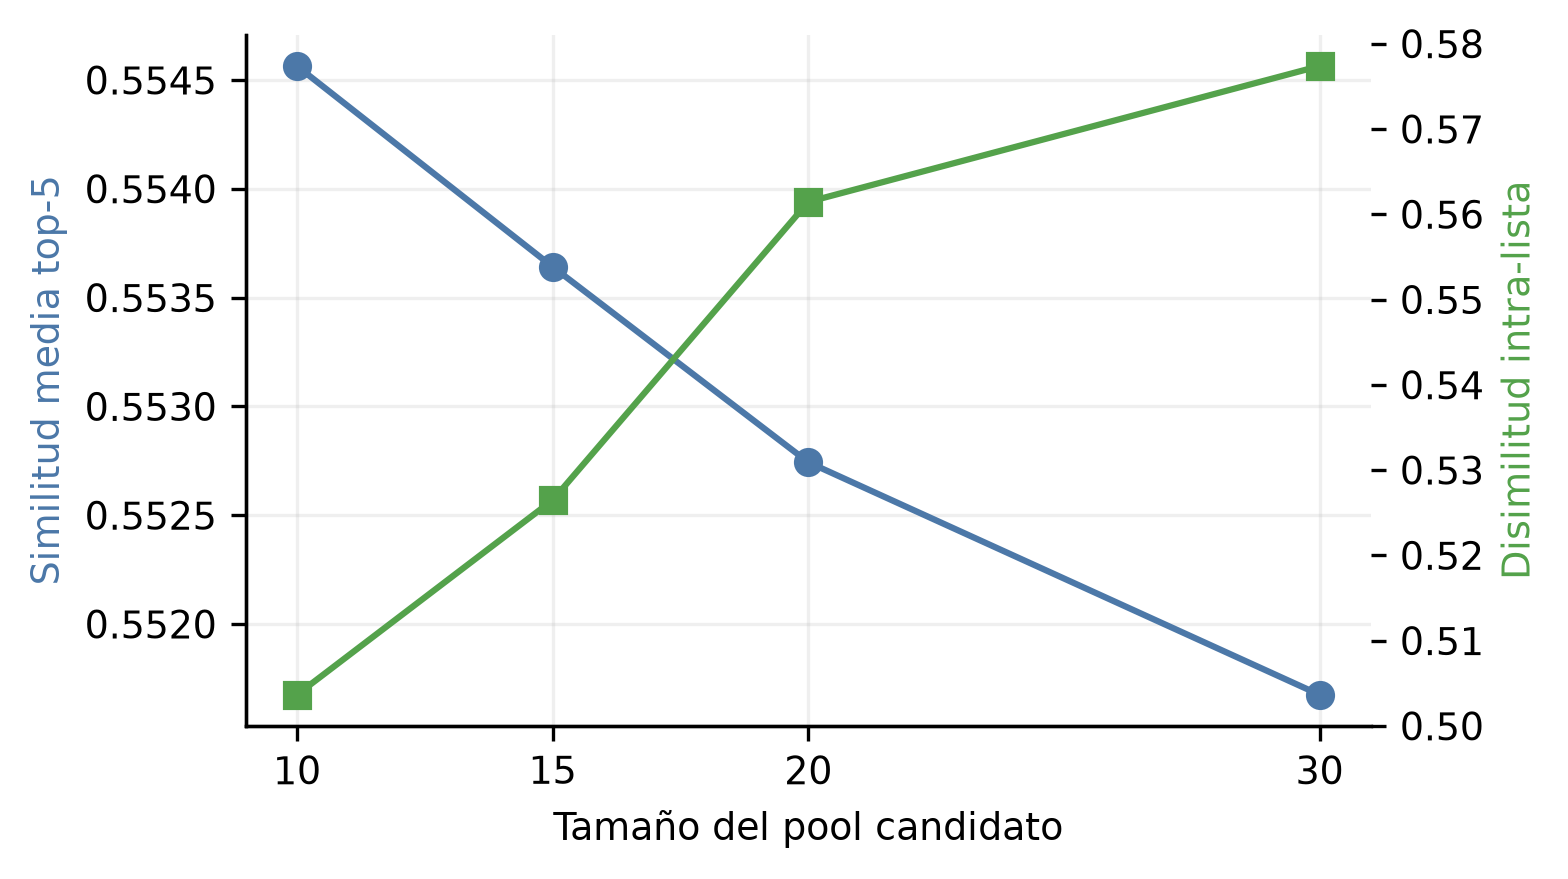
\includegraphics[width=\linewidth]{figures/sensibilidad_pool.pdf}
  \caption{Variación del pool.}
  \label{fig:pool}
\end{subfigure}
\caption{Sensibilidad de similitud y disimilitud; los ejes verticales son independientes.}
\label{fig:parameter-sensitivity}
\end{figure}

La ganancia media de \ILD{} fue positiva en las ocho tareas (\cref{fig:tasks}), desde 0,0145 en pronóstico a un paso ($n=136$) hasta 0,1475 en estimación de vida útil remanente ($n=371$). En pronóstico a un paso hubo 71 aumentos y 65 disminuciones de ILD, sin evidencia clara en Wilcoxon ($p=0{,}504$); este estrato se interpreta con cautela porque incluye tareas asignadas por defecto. Los grupos con mayor soporte fueron detección de fallas (0,0975; $n=782$), vida útil remanente (0,1475; $n=371$) y evaluación de salud (0,1026; $n=303$). La pérdida de similitud media fue $-0,0023$, $-0,0022$ y $-0,0045$, respectivamente.

\begin{figure}[H]
\centering
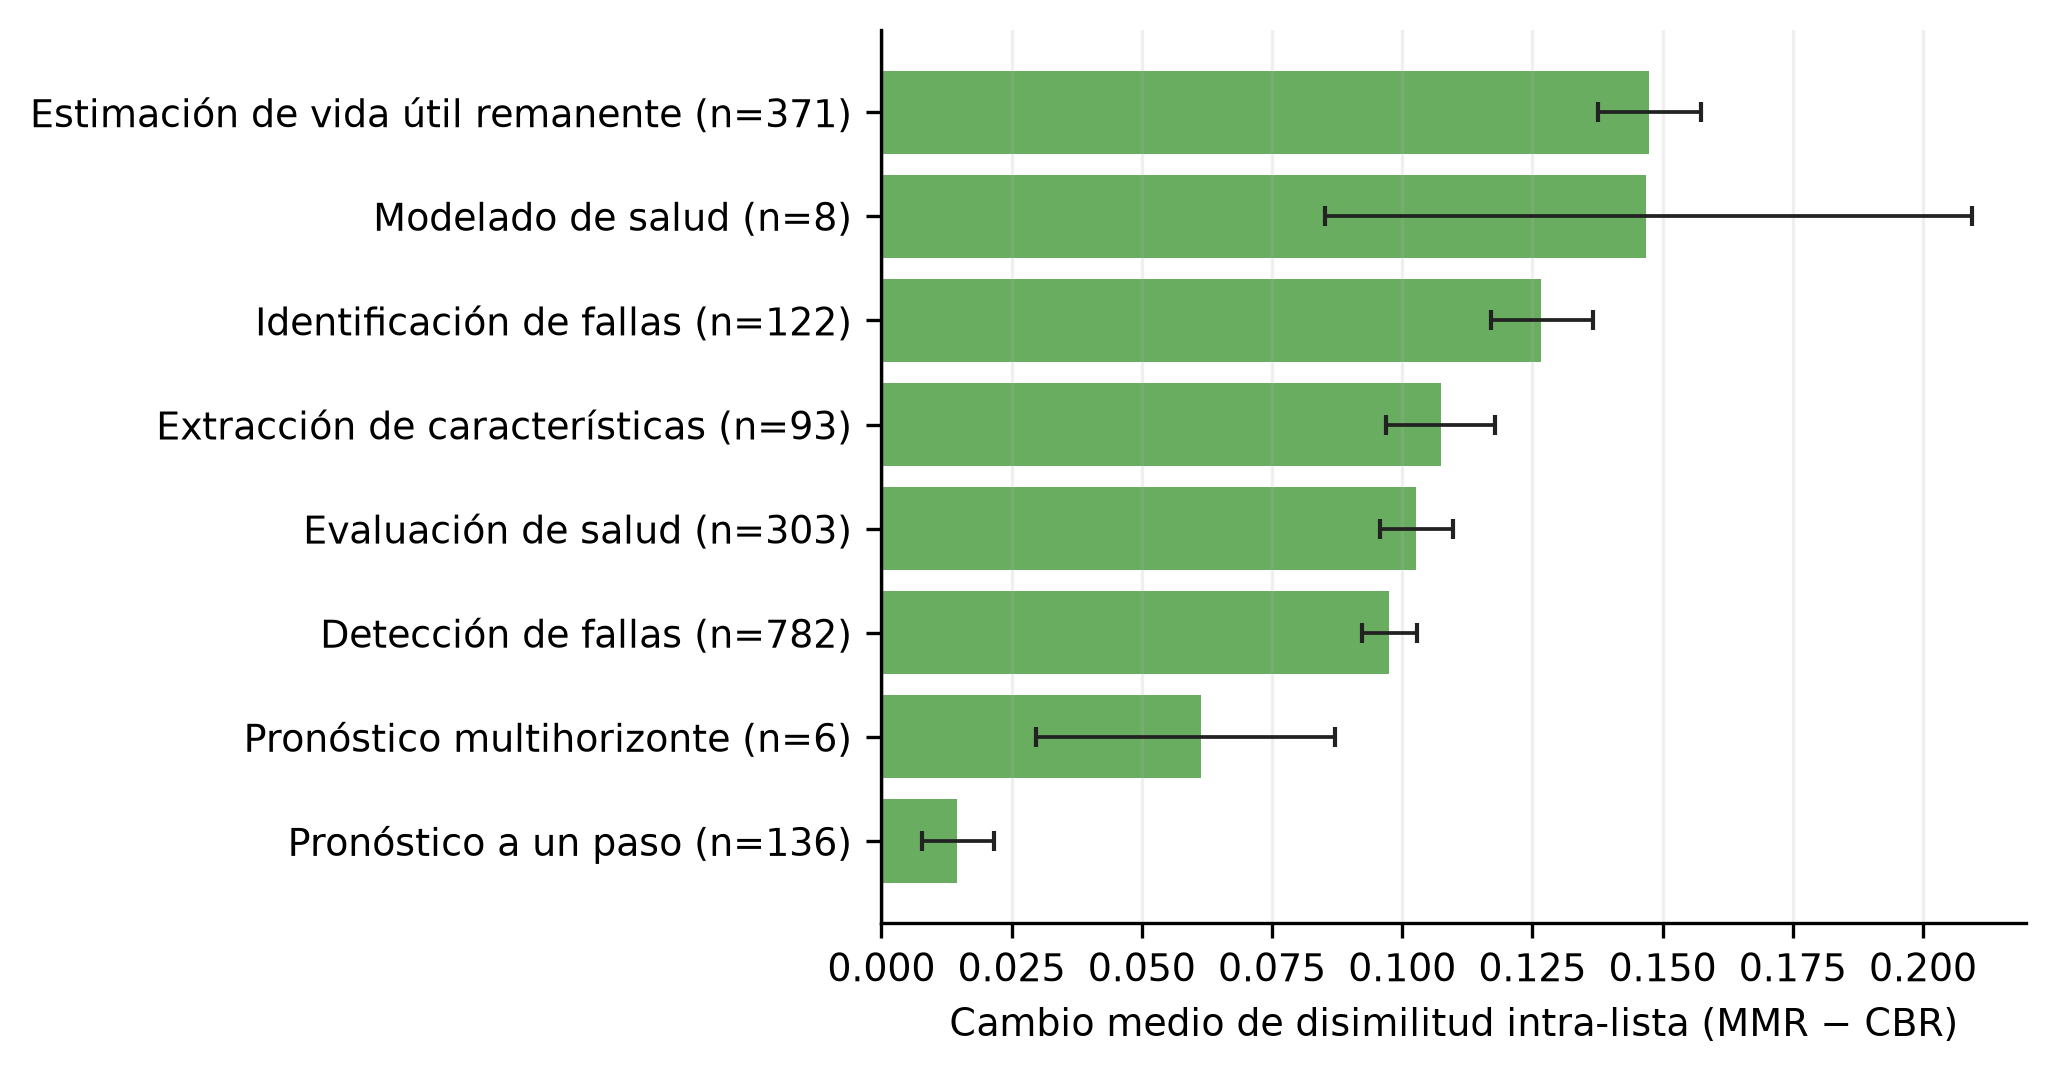
\includegraphics[width=0.88\linewidth]{figures/delta_ild_por_tarea.pdf}
\caption{Cambio medio de \ILD{} por tarea con IC95\% bootstrap. Los estratos pequeños se muestran como descripción exploratoria.}
\label{fig:tasks}
\end{figure}

\subsection{Modelo extractor y trazabilidad}

Los artefactos de \texttt{gpt-5-mini}, \texttt{gpt-5.4-mini} y \texttt{gpt-5.6-luna} tuvieron en promedio 8,74, 8,98 y 9,81 campos informativos de 19. Sus cambios de \ILD{} fueron 0,0978, 0,1002 y 0,1141. Estas diferencias son descriptivas: modelo, lote, documentos y reintentos no se asignaron aleatoriamente. Eliminar los 25 enlaces PDF--facts no exactos dejó $n = 1\,796$ y un cambio de \ILD{} de 0,1052, prácticamente igual al total (0,1049). Los 25 no exactos aislados mostraron 0,0827 y no sustentan inferencia por su tamaño.

\subsection{Ejemplo de una lista}

La \cref{tab:example} ilustra la consulta 1815, de evaluación de salud, cercana al cambio mediano. El baseline devolvió dos veces Gaussian Process Regression. MMR preservó en primer lugar los modelos de acumulación de daño y confiabilidad, y añadió regresión/reglas y estimación recursiva. La similitud media pasó de 0,5140 a 0,5112 y la \ILD{} de 0,5156 a 0,6032. El ejemplo muestra variedad léxica/taxonómica, no superioridad técnica de las alternativas.

\begin{table}[H]
\centering
\caption{Ejemplo de recomendaciones para la consulta 1815 (artefacto \texttt{facts\_1b467dde5841.ttl}).}
\label{tab:example}
\footnotesize
\begin{tabularx}{\linewidth}{clX}
\toprule
Método & Sim. & Firma de modelos \\
\midrule
CBR & 0,517 & Damage Accumulation; Structural Reliability; Physics of Failure \\
CBR & 0,517 & Echo State Network Structure \\
CBR & 0,512 & Neural Network \\
CBR & 0,512 & Gaussian Process Regression \\
CBR & 0,512 & Gaussian Process Regression \\
\midrule
CBR+MMR & 0,517 & Damage Accumulation; Structural Reliability; Physics of Failure \\
CBR+MMR & 0,517 & Echo State Network Structure \\
CBR+MMR & 0,506 & Linear Regression; Rule-Based System \\
CBR+MMR & 0,512 & Non-linear Least Squares with Dynamic Bounds \\
CBR+MMR & 0,504 & Recursive Least Squares; Recursive Maximum Likelihood \\
\bottomrule
\end{tabularx}
\end{table}

\section{Discusión}
\label{sec:discussion}

\subsection{Respuesta a las preguntas de investigación}

Para P1, la metodología produjo artefactos parseables y consultas para 1.821 documentos únicos, con manifiestos, hashes, limpieza RDF-star y sidecar de procedencia. La representación es auditable porque cada etapa deja artefactos intermedios y tablas de cobertura; sin embargo, parseabilidad y trazabilidad no equivalen a fidelidad factual.

Para P2, la transformación hacia el esquema CBR fue operativamente posible, pero no preservó los 19 campos por igual. La consulta efectiva se apoyó sobre todo en tarea, activo, variables y año; varios campos quedaron predeterminados o se descartaron durante la normalización, y solo 126 artefactos cumplieron todas las formas SHACL mínimas. El resultado demuestra compatibilidad operativa, no interoperabilidad semántica plena.

Para P3, la tarea downstream mostró que el reranking puede reducir redundancia con una pérdida pequeña de similitud en la escala CBR: MMR redujo de 610 a 5 las listas repetidas y aumentó 24,89\% la \ILD{} con $-0,48\%$ de similitud. No obstante, deduplicación, max-sum y DPP revelaron objetivos distintos, y la sensibilidad a $\lambda$, pool, $k$, pesos, atributos y recencia impide presentar un parámetro universal. En consecuencia, el resultado debe leerse como comportamiento algorítmico de una capa reversible de diversidad, no como evidencia de recomendaciones mejores para usuarios.

\subsection{Relación con trabajos previos}

El estudio extiende la línea \OPMAD{}--CBR \citep{MonteroJimenez2021OPMADCBR,MunozHernandez2021OntologyCBR} al automatizar consultas desde literatura, exponer pérdida de información y ejecutar el DSS por lotes. El reranking no sustituye la condensación de \citet{MunozPena2025Diversity}; la \cref{tab:cnn-mmr} delimita ambos. La comparación directa exige reconstruir la memoria CNN y sigue abierta, mientras deduplicación, max-sum y DPP sí se compararon sobre igual pool.

\begin{table}[H]
\centering
\caption{Diferencias conceptuales entre condensación CNN previa y MMR.}
\label{tab:cnn-mmr}
\small
\begin{tabularx}{\linewidth}{lXX}
\toprule
Aspecto & CNN modificado \citep{MunozPena2025Diversity} & MMR de este estudio \\
\midrule
Momento & mantenimiento de la memoria & postproceso de cada recuperación \\
Persistencia & modifica/generaliza índices & no altera casos ni similitudes CBR \\
Objetivo & tamaño, cobertura y diversidad & relevancia--diversidad de una lista \\
Parámetros & umbrales de descripción/solución & $\lambda$, pool, $k$ y pesos de solución \\
Costo recurrente & menor tras condensar, mayor preparación & cálculo voraz por consulta \\
Evidencia & 224 casos de desarrollo y 40 consultas & 263 casos históricos y 1.821 consultas automáticas \\
Límite principal & posible pérdida por generalización & dependencia del pool y de $s_{\mathrm{sol}}$ \\
\bottomrule
\end{tabularx}
\end{table}

La mejora de \ILD{} es esperable porque MMR optimiza una función relacionada. Los conteos de firmas, tipos y enfoques ofrecen vistas discretas adicionales, pero tampoco son utilidad. Una evaluación con arquitectos para medir relevancia, novedad, utilidad, tiempo, confianza y adopción permanece como trabajo futuro; no se presentan resultados humanos.

\subsection{Implicaciones de ingeniería}

La separación entre extracción, puente, recuperación y reranking permite auditar cada interfaz. El esquema fijo limita cambios silenciosos; el adaptador por lotes habilita regresión; el pool conserva puntajes; SHACL y tablas de cobertura exponen valores predeterminados. El sidecar preserva la procedencia RDF-star retirada del grafo de cálculo, aunque el puente todavía no la usa para escoger el estudio fuente.

Antes de retener automáticamente los 1.821 casos en la memoria CBR se requiere validación externa de fidelidad. En el experimento, los artículos se utilizaron como \emph{consultas}, no como nuevos casos. Incorporarlos sin desambiguar modelos, unidades y métricas amplificaría errores de extracción y redundancia.

\section{Amenazas a la validez}
\label{sec:threats}

\paragraph{Validez de constructo.}
La similitud CBR es un proxy y \ILD{} comparte $s_{\mathrm{sol}}$ con MMR. Firmas, tipos y enfoques exactos, más MAP-DPP, reducen pero no eliminan la dependencia de representación; una firma puede contener varios algoritmos y no equivale a diversidad funcional. No existe \emph{ground truth} ni evaluación humana.

\paragraph{Calidad de extracción.}
No se anotaron precisión, exhaustividad o F1; el piloto LLM no sustituye expertos. Los lotes mezclaron tres modelos y casi siempre solo tres fragmentos iniciales, por lo que métodos/resultados del PDF pueden omitirse. SHACL reveló baja conformidad completa y 335 literales inválidos. El sidecar conserva procedencia textual, pero siguen pendientes normalización de namespaces, transformación RDF 1.1 y ejecución del corpus dorado preregistrado.

\paragraph{Puente y consulta.}
El puente usa valores predeterminados y derivados: 0 para conteos, sincronización desconocida y pronóstico a un paso sin evidencia. Cuatro campos tuvieron 0\% de cobertura informativa y 121 consultas quedaron en tarea+año. En 409 artefactos se eligió el primer IRI sin prueba de ser el estudio fuente. La base de 263 casos limita cobertura; las ablaciones confirmaron que año y atributos cambian materialmente rankings.

\paragraph{Independencia.}
Hubo 1.684 firmas, pero solo 848 rankings baseline y 699 MMR; los mayores clústeres reunieron 129 y 109 consultas. El bootstrap por clúster amplió los intervalos y es el análisis conservador. Los $p$ siguen describiendo estabilidad del sistema, no inferencia poblacional.

\paragraph{Selección y generalización.}
El corpus contiene artículos 2025--2026 en inglés y PDF accesibles. La recuperación fue menor en 2026 y varió 33,3--85,5\% entre rutas de acceso; los 946 ausentes pueden sesgar el corpus. Dominio y base pertenecen a mantenimiento predictivo; otros DSS requieren nueva validación.

\paragraph{Reproducibilidad temporal.}
La recencia dependía del reloj; se fijó 2026 y la ablación mostró su impacto. La extracción LLM es estocástica y dependiente de versiones. Por ello se publican TTL canónicos, hashes, sidecar, prompts/configuración, manifiesto de software y resultados por consulta; reproducen el experimento desde artefactos, no necesariamente la generación original bit a bit.

\section{Conclusiones}
\label{sec:conclusion}

Se presentó y auditó un puente entre extracción LLM restringida por \OPMAD{}, esquema CBR, consulta CBR y diversificación. Las 1.821 consultas fueron ejecutables, pero la auditoría cuantificó que varios de los 19 campos quedaron predeterminados o se descartaron. Con $\lambda=0{,}70$, MMR aumentó \ILD{} 0,1049 y redujo de 610 a 5 las listas repetidas con $-0,0027$ de similitud. Bootstrap por clúster, pools, pesos, atributos y comparadores confirmaron un compromiso configurable, no una superioridad universal; el desglose por modelo/lote fue solo descriptivo.

La evidencia respalda interoperabilidad ejecutable y comportamiento de ranking. No respalda exactitud semántica ni valor decisional. Los siguientes pasos son eliminar valores predeterminados engañosos, identificar el estudio fuente por evidencia, convertir la procedencia a RDF estándar, comparar el reranking con memoria CNN reconstruida y, si se busca afirmar fidelidad o utilidad, ejecutar una evaluación experta independiente.

\section*{Disponibilidad de datos y código}
El suplemento incluye consulta y cribado por registro, manifiesto PDF--facts, hashes, SHACL, resultados por consulta, bootstrap por clúster, comparadores, ablaciones, sensibilidad y manifiesto de software. Incluye además las 311.559 asociaciones RDF-star en un sidecar comprimido. Los PDF no se redistribuyen por licencia. El manifiesto de 1.822 filas PDF contiene 1.797 enlaces exactos/casi exactos y 25 no exactos; al deduplicar, el análisis usa 1.796+25=1.821. Excluir los 25 no cambió la conclusión. El identificador del repositorio se añadirá al depositar la versión asociada al envío.

El experimento principal se reproduce desde los facts canónicos definiendo la ruta larga de la base en \texttt{CASEBASE}:

\begin{verbatim}
.\.venv\Scripts\python.exe scripts\compare_diversity_all_papers.py `
  --facts-glob "extraction_papers/ontocast_runs/run_*/output/facts_*.ttl" `
  --casebase-csv $env:CASEBASE --top-k 5 --pool-size 15 `
  --lambda-relevance 0.70 --query-year 2026 `
  --drop-default-synchronization `
  --output-dir .build\reproduccion_articulo
.\.venv\Scripts\python.exe paper\analysis\statistical_analysis.py
.\.venv\Scripts\python.exe paper\analysis\revision_audit.py
\end{verbatim}

\section*{Declaraciones}
\textbf{Aprobación ética:} no aplica; no participaron personas ni animales.\par
\textbf{Conflictos de interés:} los autores declaran no tener conflictos de interés.\par
\textbf{Financiación:} información anonimizada para revisión por pares.\par
\textbf{Uso de inteligencia artificial generativa:} \texttt{gpt-5-mini}, \texttt{gpt-5.4-mini} y \texttt{gpt-5.6-luna} formaron parte del método de extracción. \texttt{gpt-5.5} mediante el agente pi apoyó crítica editorial, programación de auditorías y revisión de redacción; no se usó para validar semánticamente las extracciones. Los autores verificaron referencias, código, cifras y afirmaciones y asumen responsabilidad final.

\appendix
\section{Campos de interoperabilidad}
\label{app:fields}
\begin{table}[ht]
\centering
\caption{Esquema de 19 campos y cobertura no predeterminada ($n = 1\,821$).}
\footnotesize
\begin{tabularx}{\linewidth}{rllXr}
\toprule
N.º & Campo & Tipo & Tratamiento principal & Info. \\
\midrule
1 & Reference & entero & identificador local derivado & 100,0\% \\
2 & Publication Year & entero & literal o valor 2021 predeterminado & 35,6\% \\
3 & Task & símbolo & ocho funciones o valor predeterminado & 94,8\% \\
4 & Case study & texto & primer activo etiquetado & 84,8\% \\
5 & Case study type & símbolo & genérico si falta & 0,0\% \\
6 & Input for the model & símbolo & acción/registro & 1,3\% \\
7 & Number of input variables & entero & conteo derivado & 84,6\% \\
8 & Input type & lista & etiquetas no generadas & 71,4\% \\
9 & Data Pre-processing & booleano & inferido de diseño & 71,8\% \\
10 & Model Approach & símbolo & derivado del número de modelos & 100,0\% \\
11 & Model Type & lista & clases/tipos no generados & 71,2\% \\
12 & Models & lista & modelos no generados & 76,6\% \\
13 & Online/Off-line & símbolo & sincronización o desconocida & 0,0\% \\
14 & Number of failure modes & entero & valor o cero heredado & 0,0\% \\
15 & Performance indicator & texto & valor o no reportado & 0,0\% \\
16 & Performance & texto & valor o no reportado & 0,0\% \\
17 & Complementary notes & texto & palabras clave/diseño & 81,3\% \\
18 & Study title & texto & título no generado & 47,9\% \\
19 & Publication identifier & texto & identificador o URN & 1,4\% \\
\bottomrule
\end{tabularx}
\end{table}

\FloatBarrier
\bibliographystyle{unsrtnat}
\bibliography{references}

\end{document}
